\documentclass[10pt]{article}
\usepackage[utf8]{inputenc}

\usepackage[english]{babel}
\usepackage{array}
 
\usepackage{amsthm}
\usepackage{amssymb}
\usepackage{amsmath}
\usepackage{wasysym}
\usepackage{longtable}
\usepackage{listings}
\usepackage[dvipsnames]{xcolor}
\usepackage[utf8]{inputenc}
\usepackage{multicol}
\usepackage{hyperref}

\usepackage{geometry}
 \geometry{
 a4paper,
 total={180mm,262mm},
 left=15mm,
 top=15mm,
 }
 
\theoremstyle{plain}
\newtheorem{theorem}{Theorem}[section]

\theoremstyle{definition}
\newtheorem{example}[theorem]{Example}

\theoremstyle{definition}
\newtheorem{algorithm}[theorem]{Algorithm}

\theoremstyle{definition}
\newtheorem{problem}[theorem]{Problem}

\newcommand{\R}{\mathbb{R}}
\newcommand{\Prob}{\mathbbs{P}}
\newcommand{\E}{\mathbb{E}}

\usepackage{graphicx}
\graphicspath{ {./images/} }

\usepackage{float}
\usepackage{subcaption}

\newenvironment{Figure}
  {\par\medskip\noindent\minipage{\linewidth}}
  {\endminipage\par\medskip}

\title{Solving the Word Problem}
\author{Niam Vaishnav}
\date{}

\begin{document}

\maketitle

\setlength{\columnsep}{1cm}


\begin{multicols}{2}




\setlength{\parskip}{0.5em}
\setlength{\parindent}{0em}

% -------------------------------------------------------------

\section{Introduction}

The Word Problem is a computational problem in Combinatorial Group Theory which is extremly difficult to solve in general. We will focus on solving the Word Problem for groups, however this can also be formulated for other algebras and even to sets in general. Despite its difficultly many groups have additional structures, such as graphs and automata, which means that they admit tractable solutions to the Word Problem.

% -------------------------------------------------------------

\section{Definitions}

\subsection{Group Presentations}

Firstly, a \textbf{group} is a set $G$ equipped with a binary operation $*_G: G \times G \to G$ such that $*_G$ is associative, there is an identity element $e_G \in G$ and every element $g \in G$ has an inverse $g' \in G$. 

\begin{example}
	The main example that will we will use to illustrate these algorithms is the group $D_6$, the symmetry group of the equilateral triangle. It contains 6 elements:

	$$ D_6 = \{ e, r, r^2, s, rs, rrs \} $$

	where $r$ represents a rotation by $ \frac{2 \pi}{3}$ and $s$ is a reflection in the vertical axis. This group acts on the equilateral triangle, or equivalently the set of permutations of $\{ 1, 2, 3 \}$:

	\begin{figure}[H]
		\centering
		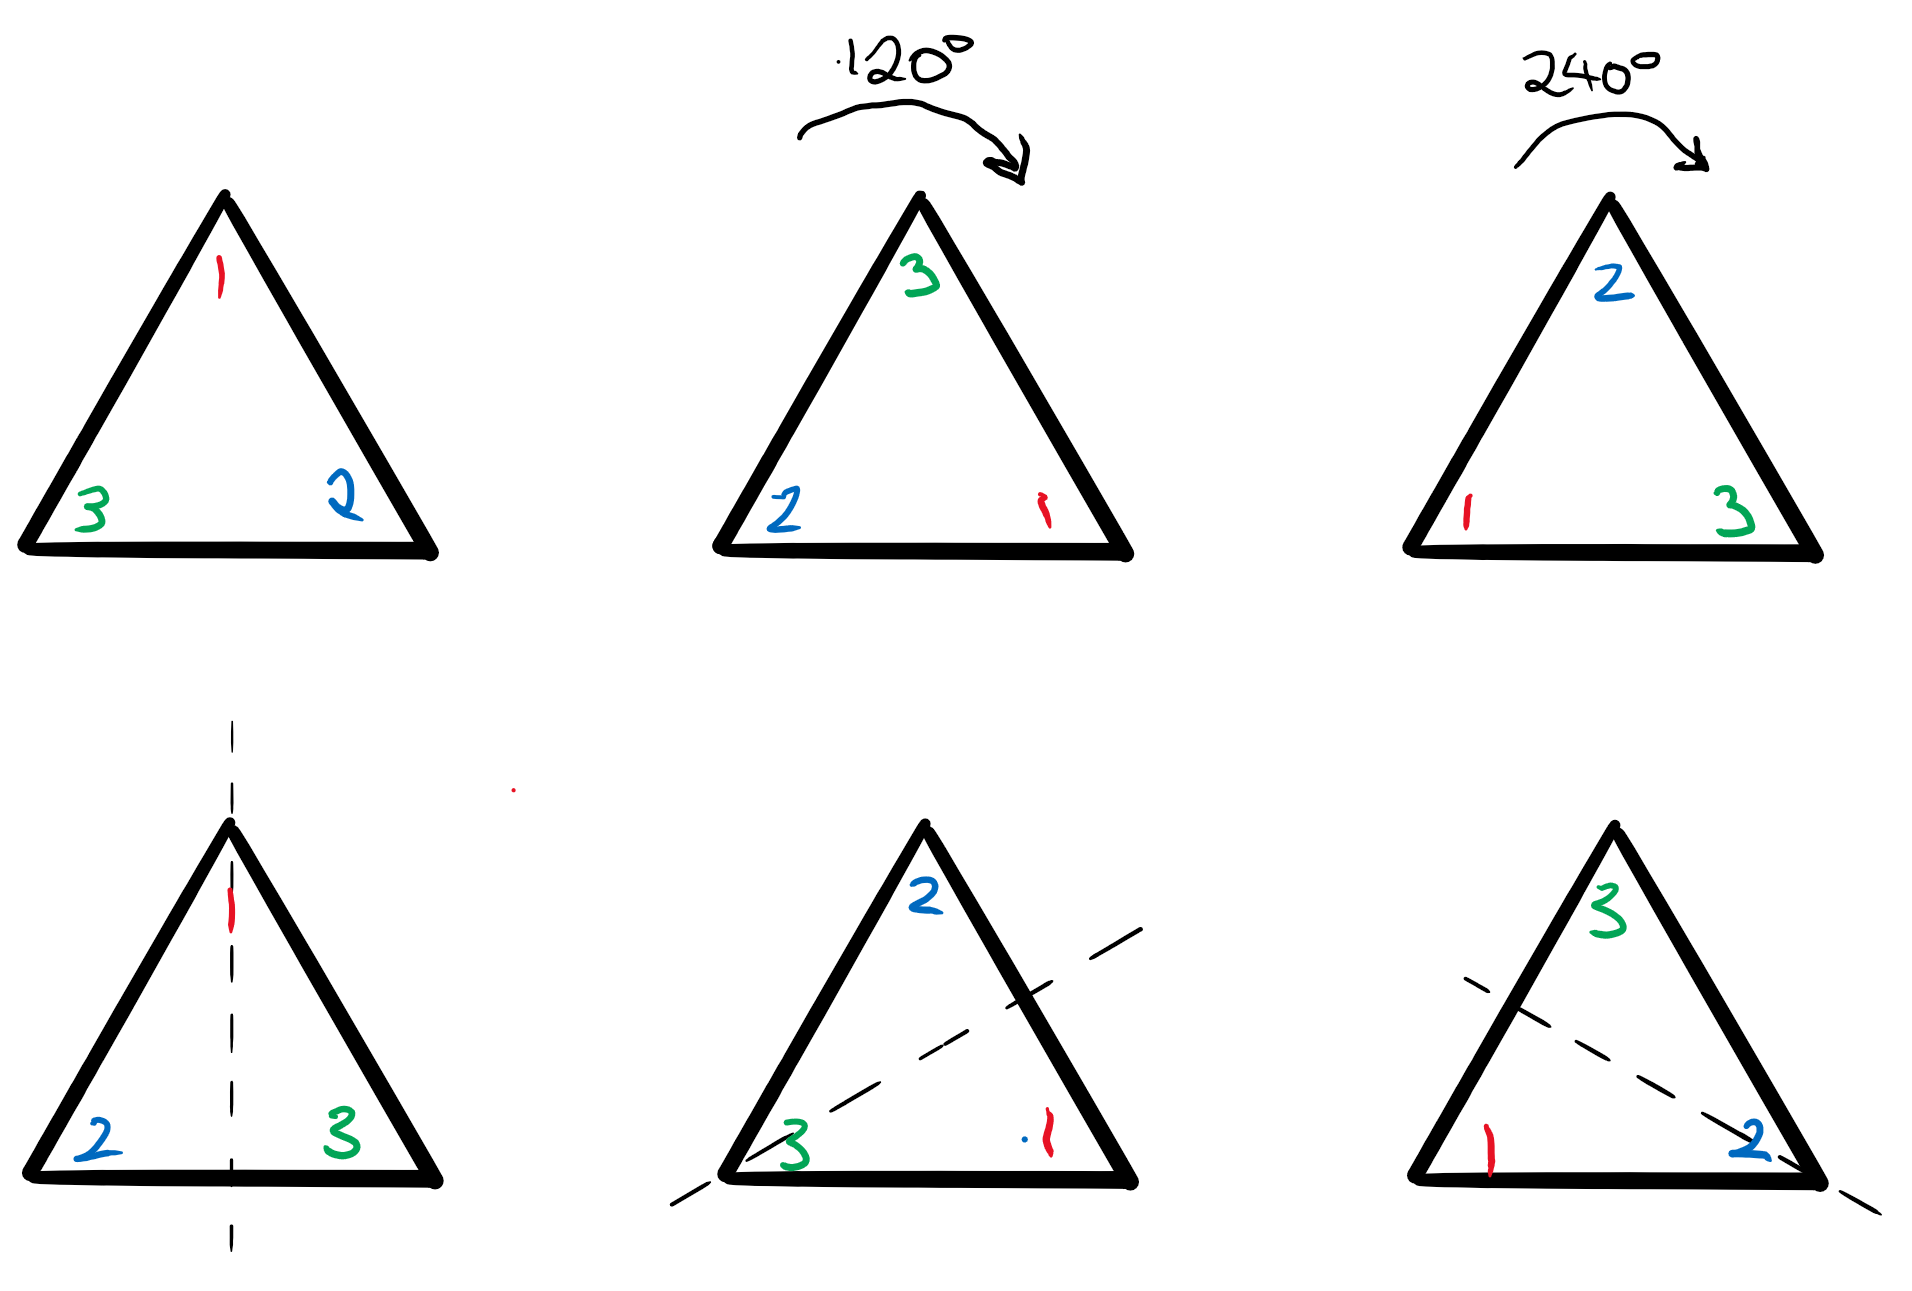
\includegraphics[scale = 0.15]{D6}
		\caption{The group $D_6$ acting on an equilateral triangle}
	\end{figure}
\end{example}

One way we can encode a group is by specifing every element in the set $G$ and the \textbf{Cayley table}, which is a matrix with rows and columns labelled by elements in $G$, and the element in cell $(g_i, g_j)$ is $g_i *_G g_j$. However, this requires $O(|G|^2)$ amount of memory to store, and so we would like to encode both the set and the Cayley table with much less information.

Let $S$ be a set of elements. The \textbf{free group} generated by $S$, written $F_S$ is the set $S^*$, where $*$ is the Kleene star. A set $S$ \textbf{generates} a group $G$ if $G \subseteq F_S$.

This is not however enough to specify a group, as there is no information about which words in the language represent the same element, such as $r$ and $r^4$ in $D_6$. Therefore, we need to specify some \textbf{relations}, which is a subset of words in $F_S$ which represent the identity element.

\begin{example}
	The group $D_6$ is generated by the set $S= \{ r, s \}$, with the relations $r^3, s^2$ and $rsrs$. This is enough to specify the group $D_6$ exactly.
\end{example}

Given a set $S$ and a set of relations $R \subseteq S^*$, a \textbf{presentation} is the quotient group:

$$ \langle S | R \rangle = F_S / N $$

where $N = R^{F_S} = \{ g^{-1} s g | g \in F_S, s \in R \}$ is the smallest normal subgroup containing every element in $R$, so that this quotient is well defined:

\begin{example}
	The presentation of the group $D_6$ is therefore:

	$$ D_6 = \langle r, s | r^3, s^2, rsrs \rangle $$
\end{example}

\subsection{Cayley Graphs}

Suppose $G$ is a group and $S \subseteq G$ is a subset of elements of $G$. The \textbf{Cayley graph} for $G$ is $\Gamma = \Gamma(G, S)$, a coloured directed graph such that:

\begin{itemize}
	\setlength\itemsep{-0.3em}
	\item $V = G$
	\item Each $s \in S$ is assigned a colour $c_s$
	\item For all $g \in G, s \in S$, $(g, gs) \in E$ with colour $c_s$
\end{itemize}

Generally, $S$ is finite, symmetric and does not contain the identity. This makes $\Gamma$ an undirected graph with no self loops. Additionally, we can equip this graph with the word metric to give the graph the structure of a metric space, giving it additional geometric properties.

The graph depends on the subset of elements of $S$:

\begin{example}
	For the group $D_6$, with the standard generating set of $\{ r, s \}$ we get the Cayley graph in Figure 2a. However, if instead we use the set $\{ s, rs \}$ which also generates $D_6$, we get the Cayley Graph in Figure 2b.

	\begin{figure*}[t]
		\centering
		\begin{subfigure}{.3\textwidth}
			%\centering
			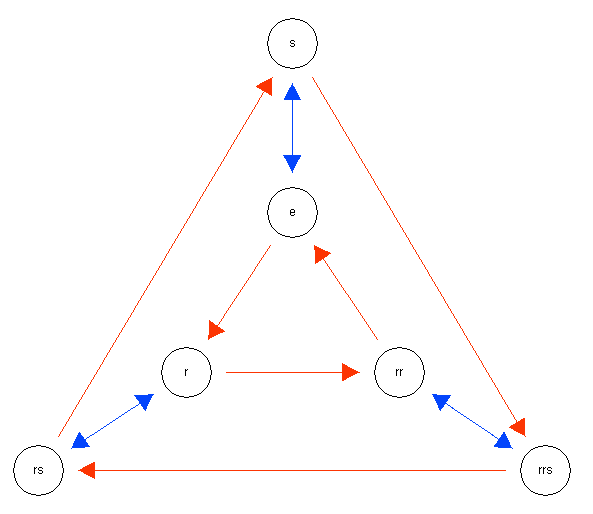
\includegraphics[scale = 0.3]{D6_gen1}
			\caption{Generating Set: $\{ \textcolor{red}{r}, \textcolor{blue}{s} \}$}
			\label{fig2:sub1}
		\end{subfigure}%
		\begin{subfigure}{.3\textwidth}
			%\centering
			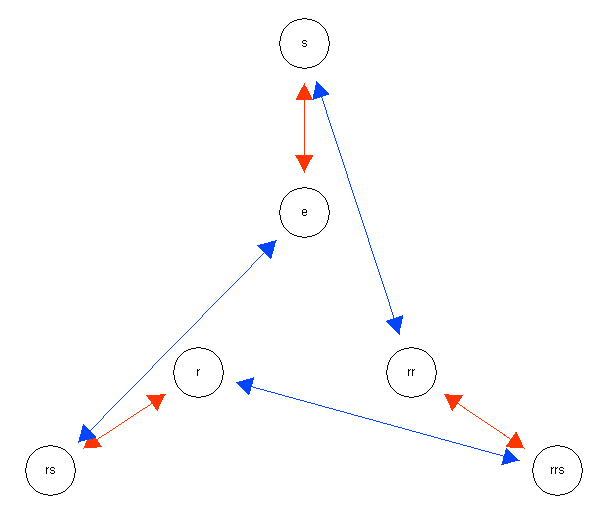
\includegraphics[scale = 0.3]{D6_gen2}
			\caption{Generating Set: $\{ \textcolor{red}{s}, \textcolor{blue}{rs} \}$}
			\label{fig2:sub2}
		\end{subfigure}
		\begin{subfigure}{.3\textwidth}
			%\centering
			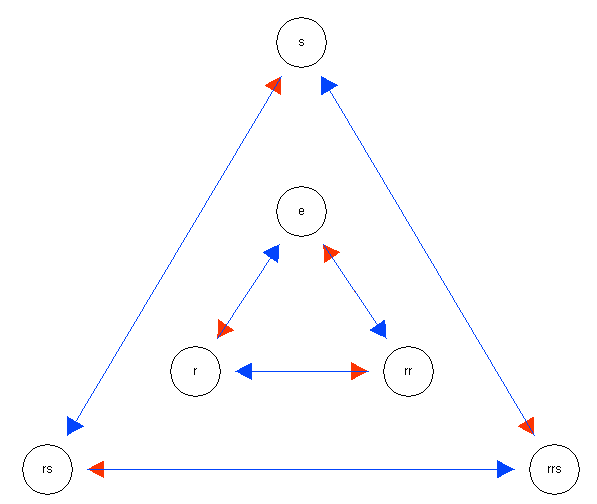
\includegraphics[scale = 0.3]{D6_gen3}
			\caption{Generating Set: $\{ \textcolor{red}{r}, \textcolor{blue}{rr} \}$}
			\label{fig2:sub3}
		\end{subfigure}
		\caption{Cayley graphs of the group $D_6$}
	\end{figure*}
\end{example}

If we do not insist that $S$ generates the set, then the Cayley graph $\Gamma$ will be disconnected. More specifically, the connected components of $\Gamma$ will be the cosets of $S^G$ in $G$. 

\begin{example}
	In $D_6$, if $S = \{ r, rr \}$, then we get the Cayley graph in Figure 2c. This has two connected components: $\{ e, r, rr \}$ and $\{ s, rs, rrs \}$, representing the cosets $S^{D_6}$ and $s*S^{D_6}$.
\end{example}

This gives an algorithm for determining if a set $S$ generates a group:

\begin{algorithm}
	Take $G$ a group and $S \subseteq G$. Let $\Gamma = \Gamma(G, S)$ and consider the uncoloured graph $\Gamma_u$. We can use a depth first search to check if $\Gamma_u$ is connected:

	\begin{enumerate}
		\setlength\itemsep{0em}
		\item Run DFS-Visit from $e$, the identity element
		\item Check if any verticies have not been visited. If so, reject. Otherwise accept.
	\end{enumerate}
\end{algorithm}

% -------------------------------------------------------------

\section{The Word Problem}

The Word Problem for groups was first proposed by Max Dehn in 1911 \cite{Dehn}. He believed that it was an important area of study along with other computational problems in Group Theory such as the Conjugacy Problem and the Isomorphism Problem. It is a very difficult problem in general, as it was proven to be undecidable in 1955 by Pyotr Novikov \cite{Novikov}. This means that there exists groups $G$ such that it is impossible to solve the Word Problem.

There are two equivalent formulations of the Word Problem, both as decision problems:

\begin{problem}
	\textbf{(Word Problem for Groups, 1st Form)} Let $G$ be a group generated by a set $X$. Let $\Sigma = X \cup X^{-1}$. The Word Problem is given two words $w_1, w_2 \in \Sigma^*$, we want to determine if they represent the same element in $G$, so $w_1 =_G w_2$.
\end{problem}

\begin{problem}
	\textbf{(Word Problem for Groups, 2nd Form)} Let $G$ be a group generated by a set $X$. Let $\Sigma = X \cup X^{-1}$. The Word Problem is given a words $w \in \Sigma^*$, we want to determine if it represent the identity element in $G$. This form can be specified easily as a language that a Turing machine needs to recognise:

		$$ L = \{ l \in \Sigma^* | l =_G e_G \} $$
\end{problem}

There is an even harder problem where the group is now an input to the problem which is RE-complete, which means that every other computable problem can be reduced to this problem, making it a representative of the hardest problems that are computable:

\begin{problem}
	\textbf{(Uniform Word Problem)} Given a group $G$, given as a presentation $\langle S | R \rangle $, and two words $\Sigma^*$, we want to determine if they represent the same element in $G$.
\end{problem}

Whilst this problem is unsolvable, many groups do have a solvable word problem, for example all finite groups. There is a stronger result in terms of regular languages and deterministic finite automata \cite{RegularWords}:

\begin{theorem}
	Suppose $G$ is a finitely generated group. If $G$ is finite, then the Word Problem is regular.
\end{theorem}

\begin{proof}
	Consider the Cayley Graph $\Gamma$ of $G = \langle S | R \rangle$. We can construct a deterministic finite automaton:

	\begin{itemize}
		\setlength\itemsep{-0.3em}
		\item $Q = G$
		\item $\Sigma = S$
		\item For all $g \in G, s \in S$, $\delta(g, s) = gs$
		\item $q_0 = e$
		\item $F = \{ e \}$ 
	\end{itemize}	

	which accepts precisely the words that represent the words that represent the identity element. This construction can be seen for $D_6$ in Figure 3:

	\begin{figure}[H]
		\centering
		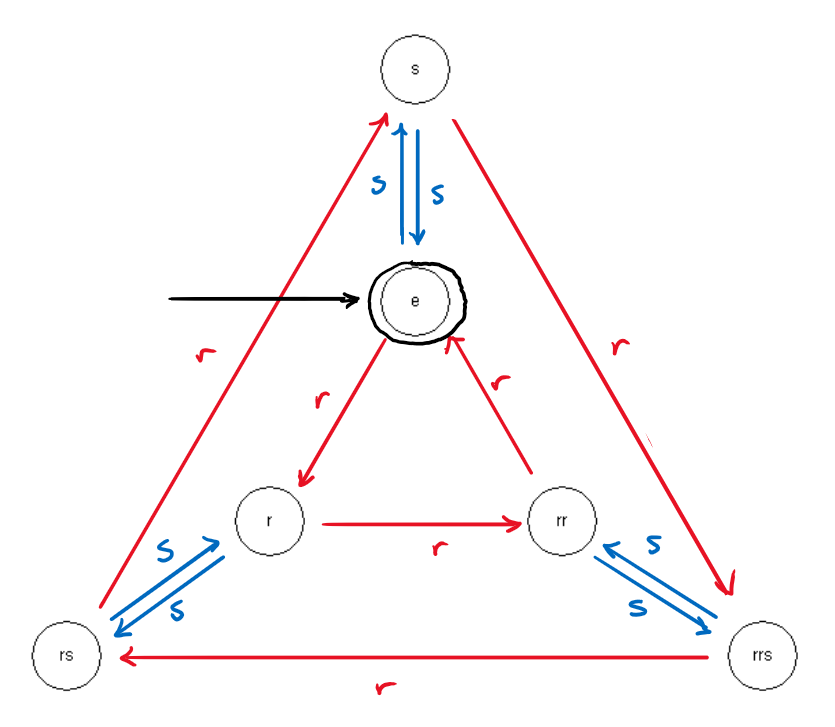
\includegraphics[scale = 0.3]{DFA}
		\caption{The group $D_6$ acting on an equilateral triangle}
	\end{figure}
\end{proof}

This theorem can be extended to an equivalence, as if the word problem is finitely generated then it must also be finite. There is an analagous theorem for context free languages \cite{RegularWords}:

\begin{theorem}
	 If $G$ is a finitely generated group, then the word problem is context free if and only if it is virtually free.
\end{theorem}

This gives us a strategy for solving the Word Problem: given a presentation, we need to find the Cayley graph of the group. This is the basis of the next algorithm:

% -------------------------------------------------------------

\section{Todd Coxeter Algorithm}

\subsection{General Algorithm}

The \textbf{Todd Coxeter Algorithm} was created in 1936 to solve a generalisation of the Word Problem:

\begin{problem}
	\textbf{(Coset Enumeration Problem)} Let $G$ be a group and $H$ be a subgroup of G, both given as presentations. We want to count the cosets of $H$ in $G$.
\end{problem}

There is similarly an extension to the Cayley graph, called the \textbf{Schreier graph} for a $G$-set $S$ and generating set $X$, $\Gamma = (V, E)$ where:

\begin{gather*}
	V = S \\
	E = \{ (s, gs) : g \in X, s \in S \}
\end{gather*}

If $S = G$, then $\Gamma$ is the Cayley graph for $G$. Furthermore, if $S = G/H$ is the set of cosets of some subgroup $H$, then $S$ is a $G$-set and hence has a Schreier graph. This is the graph which the Todd Coxeter algorithm produces in general.

The Word Problem reduces to the Coset Enumeration Problem, as we can take $H = \langle e \rangle$ so that $G/H \simeq G$. Therefore the solution enumerates the elements of $G$ and create the Schrier graph, which in this case is the Cayley graph, provided $G$ is finite. We will focus on this special case, with the slight abuse of notation taking $g$ to mean the coset $g \langle e \rangle$.

The formal version of the general Todd-Coxeter algorithm is \cite{ToddCoxeter}:

\begin{algorithm}
	\textbf{(Todd Coxeter Algorithm)} Given $G = \langle X | R \rangle$ and $ H = \langle Y \rangle $ such that $H \leq G$:

	\begin{enumerate}
		\setlength\itemsep{0em}
		\item Begin with the Cayley graph of the free group $F = \langle X \rangle$, where all the vertices are unmarked and unlabelled, except $e$ which is labelled with a 1.
		\item For each generator in $Y$, follow the path from $e$, labelling the unlabelled verticies with fresh integers. The final vertex is identified with $e$.
		\item For each labelled and unmarked vertex $s$:
			\begin{enumerate}
				\setlength\itemsep{0em}
				\item Label $s$ with a fresh integer
				\item For eery $x \in X$, label $xs$ and $x^{-1} s$ with fresh integers
				\item For every relation in $R$, follow the path from $s$ and identify the end of the path with $s$
				\item Mark s
			\end{enumerate}	
	\end{enumerate}

	To identify two verticies, we remove the vertex with the greater integer label, and move all the edges from the removed vertex to the remaining vertex.
\end{algorithm}

\begin{example}
	In the case where $H$ is trivial, the second step is not required. Consider the algorithm executed on the group $ D_6 = \langle r, s | r^3, s^2, rsrs \rangle $. In order to speed up the algorithm, it is helpful to add the rules $r r^{-1}$ and $s s^{-1}$
	
	Figure 4 shows the first steps of the algorithm.

	\begin{figure*}[p]
		\centering
		\begin{subfigure}{.4\textwidth}
			\centering
			
\includegraphics[scale = 0.55]{TC1}
			\caption{We start with a single node $0$, representing the identity element.}
			\label{fig4:sub1}
		\end{subfigure}%
		\begin{subfigure}{.4\textwidth}
			\centering
			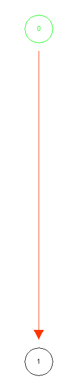
\includegraphics[scale = 0.55]{TC2}
			\caption{The first rule we add is $r^-1 r$, adding two new nodes but identifying the second with the identity. We also add a red arrow representing premultiplication by $r$.}
			\label{fig4:sub2}
		\end{subfigure}

		\begin{subfigure}{.4\textwidth}
			\centering
			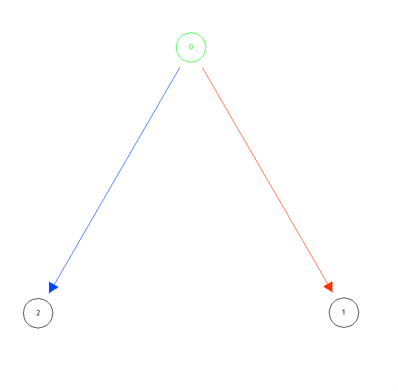
\includegraphics[scale = 0.55]{TC3}
			\caption{The next rule is $s^-1 s$, which has a very similar effect as the previous rule.}
			\label{fig4:sub3}
		\end{subfigure}
		\begin{subfigure}{.4\textwidth}
			\centering
			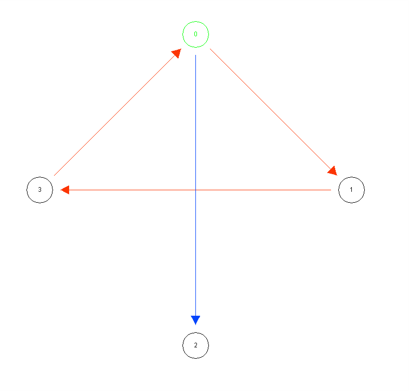
\includegraphics[scale = 0.55]{TC4}
			\caption{Now we add the rule $r^3$, causing us to add a new node from node $1$ along a red arrow. Again the final node is identified with the identity.}
			\label{fig4:sub4}
		\end{subfigure}

		\begin{subfigure}{.4\textwidth}
			\centering
			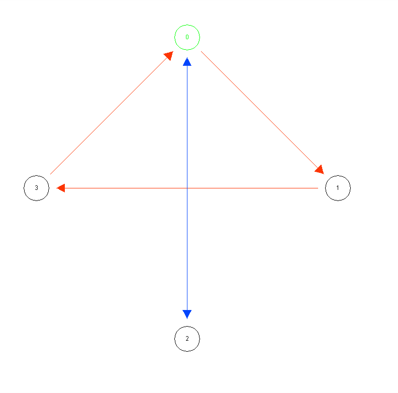
\includegraphics[scale = 0.55]{TC5}
			\caption{Next we add the rule $s^2$, which results in no new nodes added. Instead, an extra edge from node $2$ to node $0$ is added, as we now identify $b^2$ with $e$.}
			\label{fig4:sub5}
		\end{subfigure}
		\begin{subfigure}{.4\textwidth}
			\centering
			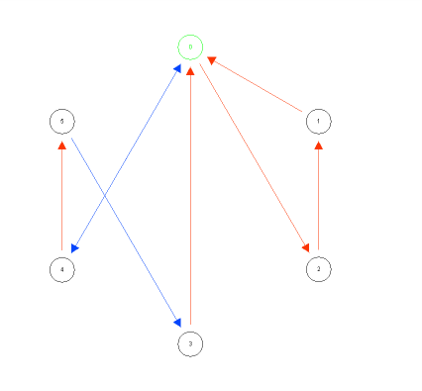
\includegraphics[scale = 0.55]{TC6}
			\caption{The final rule we need to add is $rsrs$. To do this we need to add two new nodes.}
			\label{fig4:sub6}
		\end{subfigure}

		\caption{The first 6 iterations of the Todd Coxeter algorithm on the input presentation $\langle \textcolor{red}{r}, \textcolor{blue}s | r^3, s^2, rsrs \rangle$. The edges representing multiplication by $r^{-1}$ and $s^-{1}$ have not been drawn for simplicity. Directed edges also represent premultiplication by the corresponding generator.}
	\end{figure*}

\end{example}

For termination, each vertex has a label which is monotonic decreasing, and so must eventually stabilise. Therefore if $G$ is finite, then the graph has no more than $|G|$ verticies, which have no more than $|G||X|$ neighbours, which must converge in finite time. This does not however hold if $|G|$ is infinite, there is always a graph $\Gamma_\infty$ which this sequence of graphs is converging to, but it may not do so in finite time. \cite{ToddCoxeter}

\subsection{Implementation}

This implementation has been adapted from \cite{ToddCoxeter}, and a scala version can be found PUT GITHUB HERE.

To implement this algorithm we cannot store the infinite Cayley graph of the free group, but we only need to store the section which has already been labelled, and we assume that the rest of the graph is a tree.

Each time we access a previously unvisited vertex $n$, we add a new entry to an array called \textcolor{blue}{idents} with a fresh integer. We also store a 2 dimensional array \textcolor{blue}{neighbours}, where \textcolor{blue}{neighbours[i]} stores the identities of the verticies $g * i$ for every $g \in X$, the generating set.

The value \textcolor{blue}{idents[n]} will store the smallest identity of a vertex which has been identified with $n$. In order to run the algorithm, we iterate through the elements in \textcolor{blue}{idents} in order, making a loop for each of the relations with the \textcolor{blue}{unify} function, which recusively updates the \textcolor{blue}{idents} array.

We know that this algorithm must terminate, and this is achieved when we reach the end of the \textcolor{blue}{idents} array. Once this has occured, we can reconstruct the Cayley diagram by taking a representative of each value in \textcolor{blue}{idents} which has a full row in \textcolor{blue}{neighbours} to determine where the edges in the graph should go.

\newpage

% -------------------------------------------------------------



\section{Knuth Bendix Algorithm}

\subsection{Automatic Groups}

DEFINITION FROM https://arxiv.org/pdf/math/9810190.pdf

A group $G = \langle A | R \rangle$ is \textbf{automatic} if there exists deterministic finite automata $W$ and $M_a$ for all $a \in A \cup \{ \$s \}$ such that:

\begin{enumerate}
	\item $W$ has input alphabet $A$, and for each $g \in G$, there is at least one $w \in A^*$ with $w \in \mathcal{L}(W)$ and $w \equiv_G g$
	\item For $a \in A \cup \{ \$ \}$, $M_a$ has input alphabet $(A^\dagger \times A^\dagger)^*$, and $(v^\dagger, w^\dagger) \in \mathcal{L}(M_a)$ if and only if $v, w \in \mathcal{L}(W)$ and $va \equiv_G w$
\end{enumerate}

Where $ \$ $ is a dummy symbol and $v^\dagger, w^\dagger$ are the words $v, w$ padded with $ \$ $ so that they have the same length.

The automaton $W$ is called the \textbf{word acceptor}, as it accepts at least one representative of each element of the group. The automata $M_a$ are called the \textbf{multiplier automata}.

\begin{example}
	All finite groups are automatic. The word acceptor can be constructed as the language $\mathcal{L}(W)$ can be taken to be the set of words in the finite group, and hence is finite and therefore regular.

	To construct a multiplier automaton for $g \in G$, we can use the product construction on two copies of the Cayley diagram (as a DFA in Theorem 3.4 CHECK THIS), in order to run both $v^\dagger$ and $w^\dagger$ simultaneuosly. The accepting states are $(a, b)$ such that $ag \equiv_G b$.
\end{example}

FROM file:///C:/Users/Niam/Downloads/automatic-final%20(1).pdf

The tuple $(A, \mathcal{L}(W))$ is called the \textbf{automatic structure} of the group $G$. Specifying this unambigously defines the automata $W$ and $M_a$.

We can use these to solve the word problem in quadratic time:

FROM file:///C:/Users/Niam/Downloads/D.%20B.%20A.%20Epstein%20-%20Word%20Processing%20in%20Groups%20(1992,%20CRC%20Press)%20-%20libgen.lc.pdf (Word Processing in Groups)

\begin{theorem}
	Let $G$ be an automatic group and $(A,\mathcal{L})$ be an automatic structure for $G$. For any word $w$ over $A$, we can find a string in $\mathcal{L}$ representing the same element of $G$ as $w$, in time propertional to the length of $w$.
\end{theorem}

Hence if we know some word $e$ representing the identity element, we can check if a word $w$ represents the identity element as well by finding a string in $\mathcal{L}$ representing $w$, and then using the automaton $M_{\$}$.

\subsection{Constructing W}

Alternatively, we can also solve the word problem by only using the word acceptor $W$, by using it to reduce words into a canonical form. However, it remains to construct this automaton from the presentation of the group. One way we can do this is to construct $W$ so that it rejects a word if any of the left hand sides of the relations appear in the word, as that would mean that the word could be reduced.

\begin{example}
	Consider the group $G = \langle a, b | bab = aba \rangle$. We can then construct the automaton Figure 5 which will accept any word that does not contain $bab$. We can see this by looking at which states are reachable as we read the string $bab$:

	$$ \{ S_1, S_2, S_3, S_4 \} \xrightarrow{b} \{ S_2, S_4 \} \xrightarrow{a} \{ S_3, S_4 \} \xrightarrow{b} \{ S_4 \} $$

	So we are guarenteed to end up in the rejecting state $S_4$.

	We can then use this to reduce the input word $bbab$, as when we reach the state $S_4$, we know we have just read the string $bab$. We can then go back to the state we were in before reading $bab$, replace $bab$ with $aba$ and then continue reading the word. 
	
	We continue this until we reach the end of the word, at which point we cannot reduce it anymore. This means that $bbab$ reduced to $abaa$.

	\begin{figure*}[t]
		\centering
		% 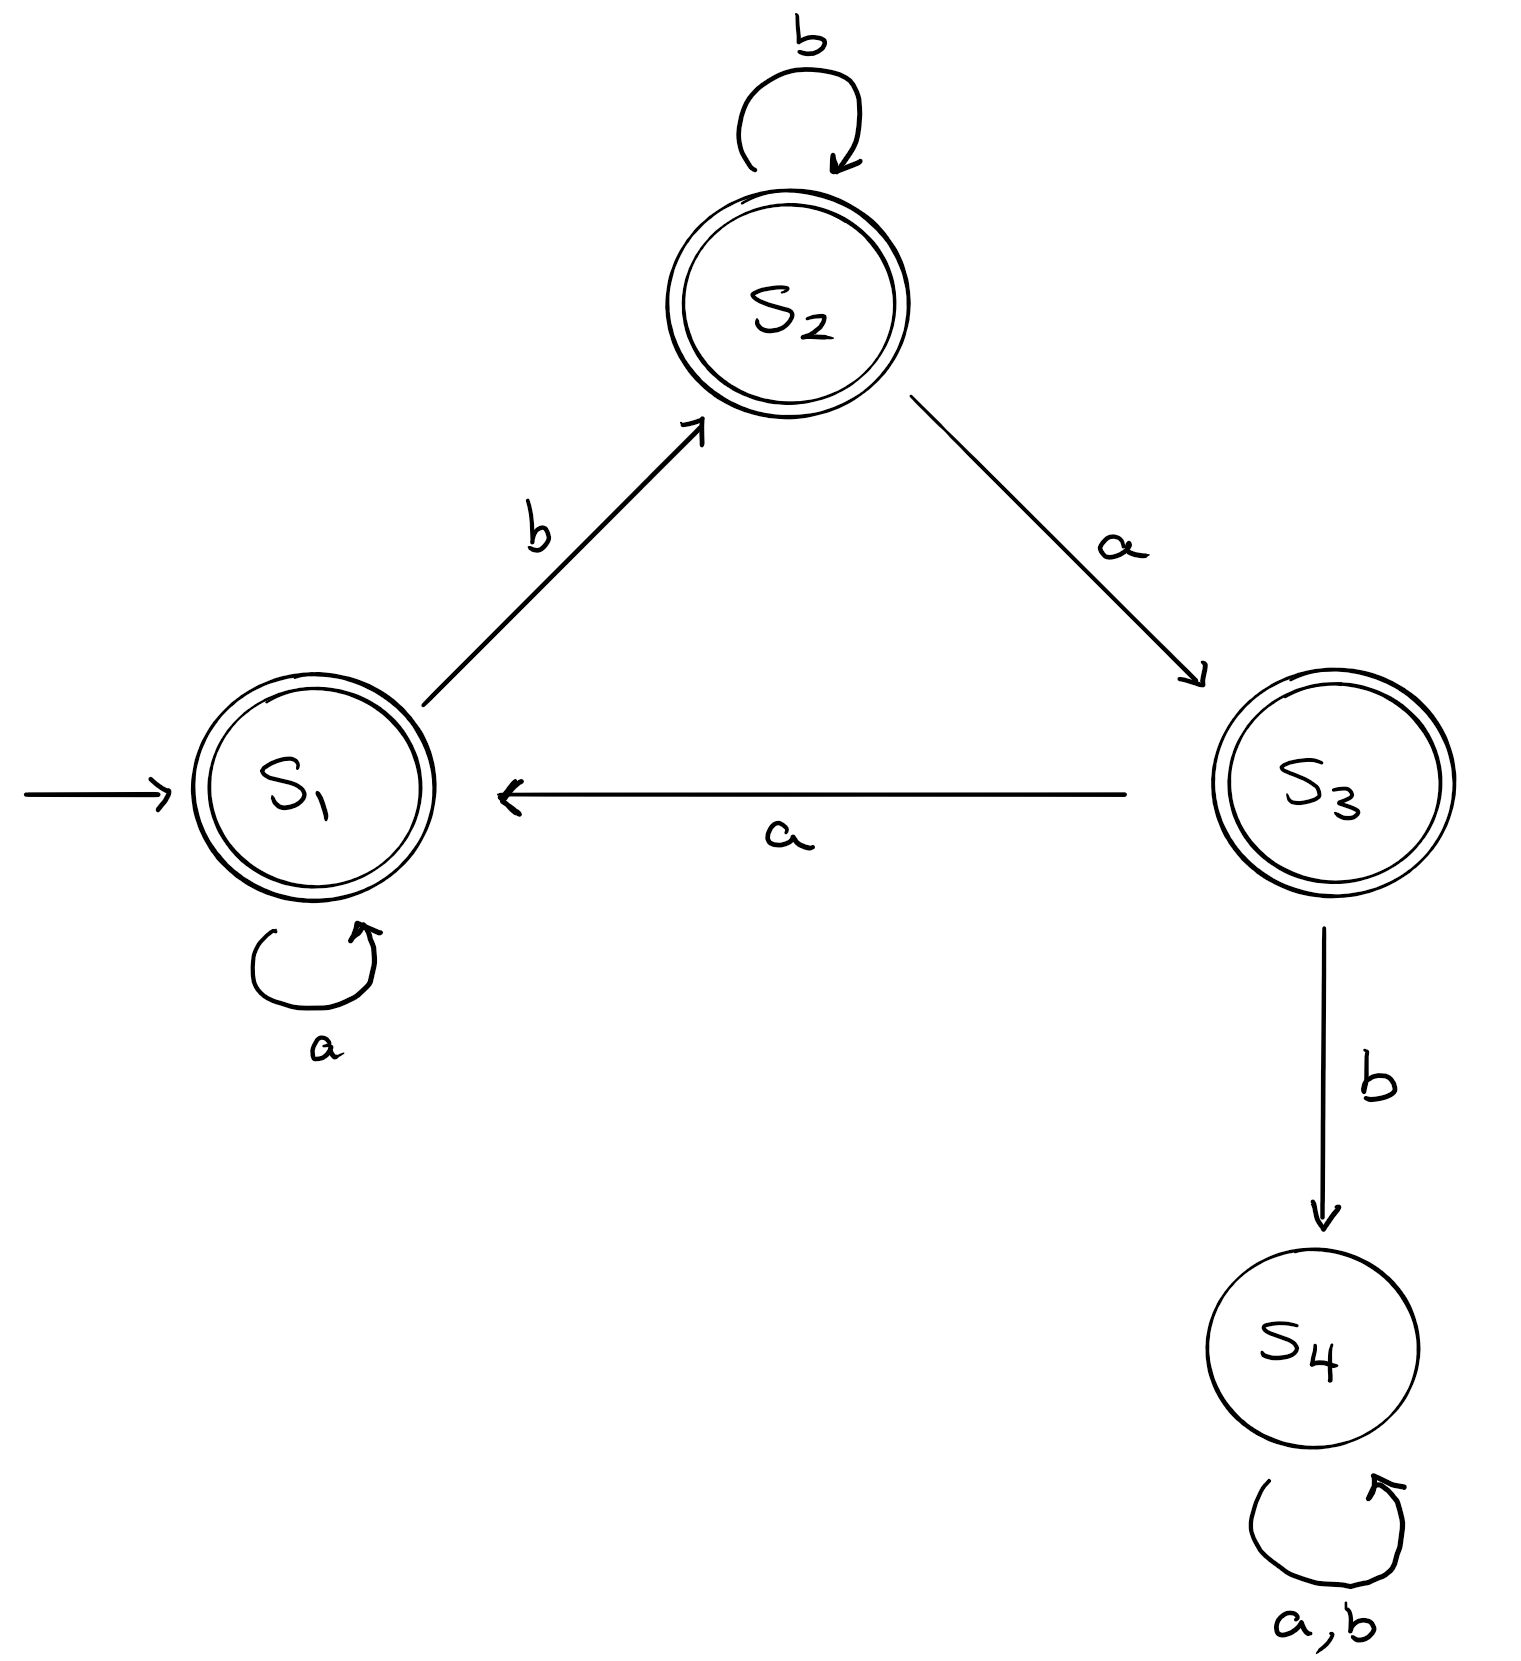
\includegraphics[scale = 0.5]{Word Acceptor.png}
		% \caption{The group $D_6$ acting on an equilateral triangle}

		\begin{subfigure}{.5\textwidth}
			%\centering
			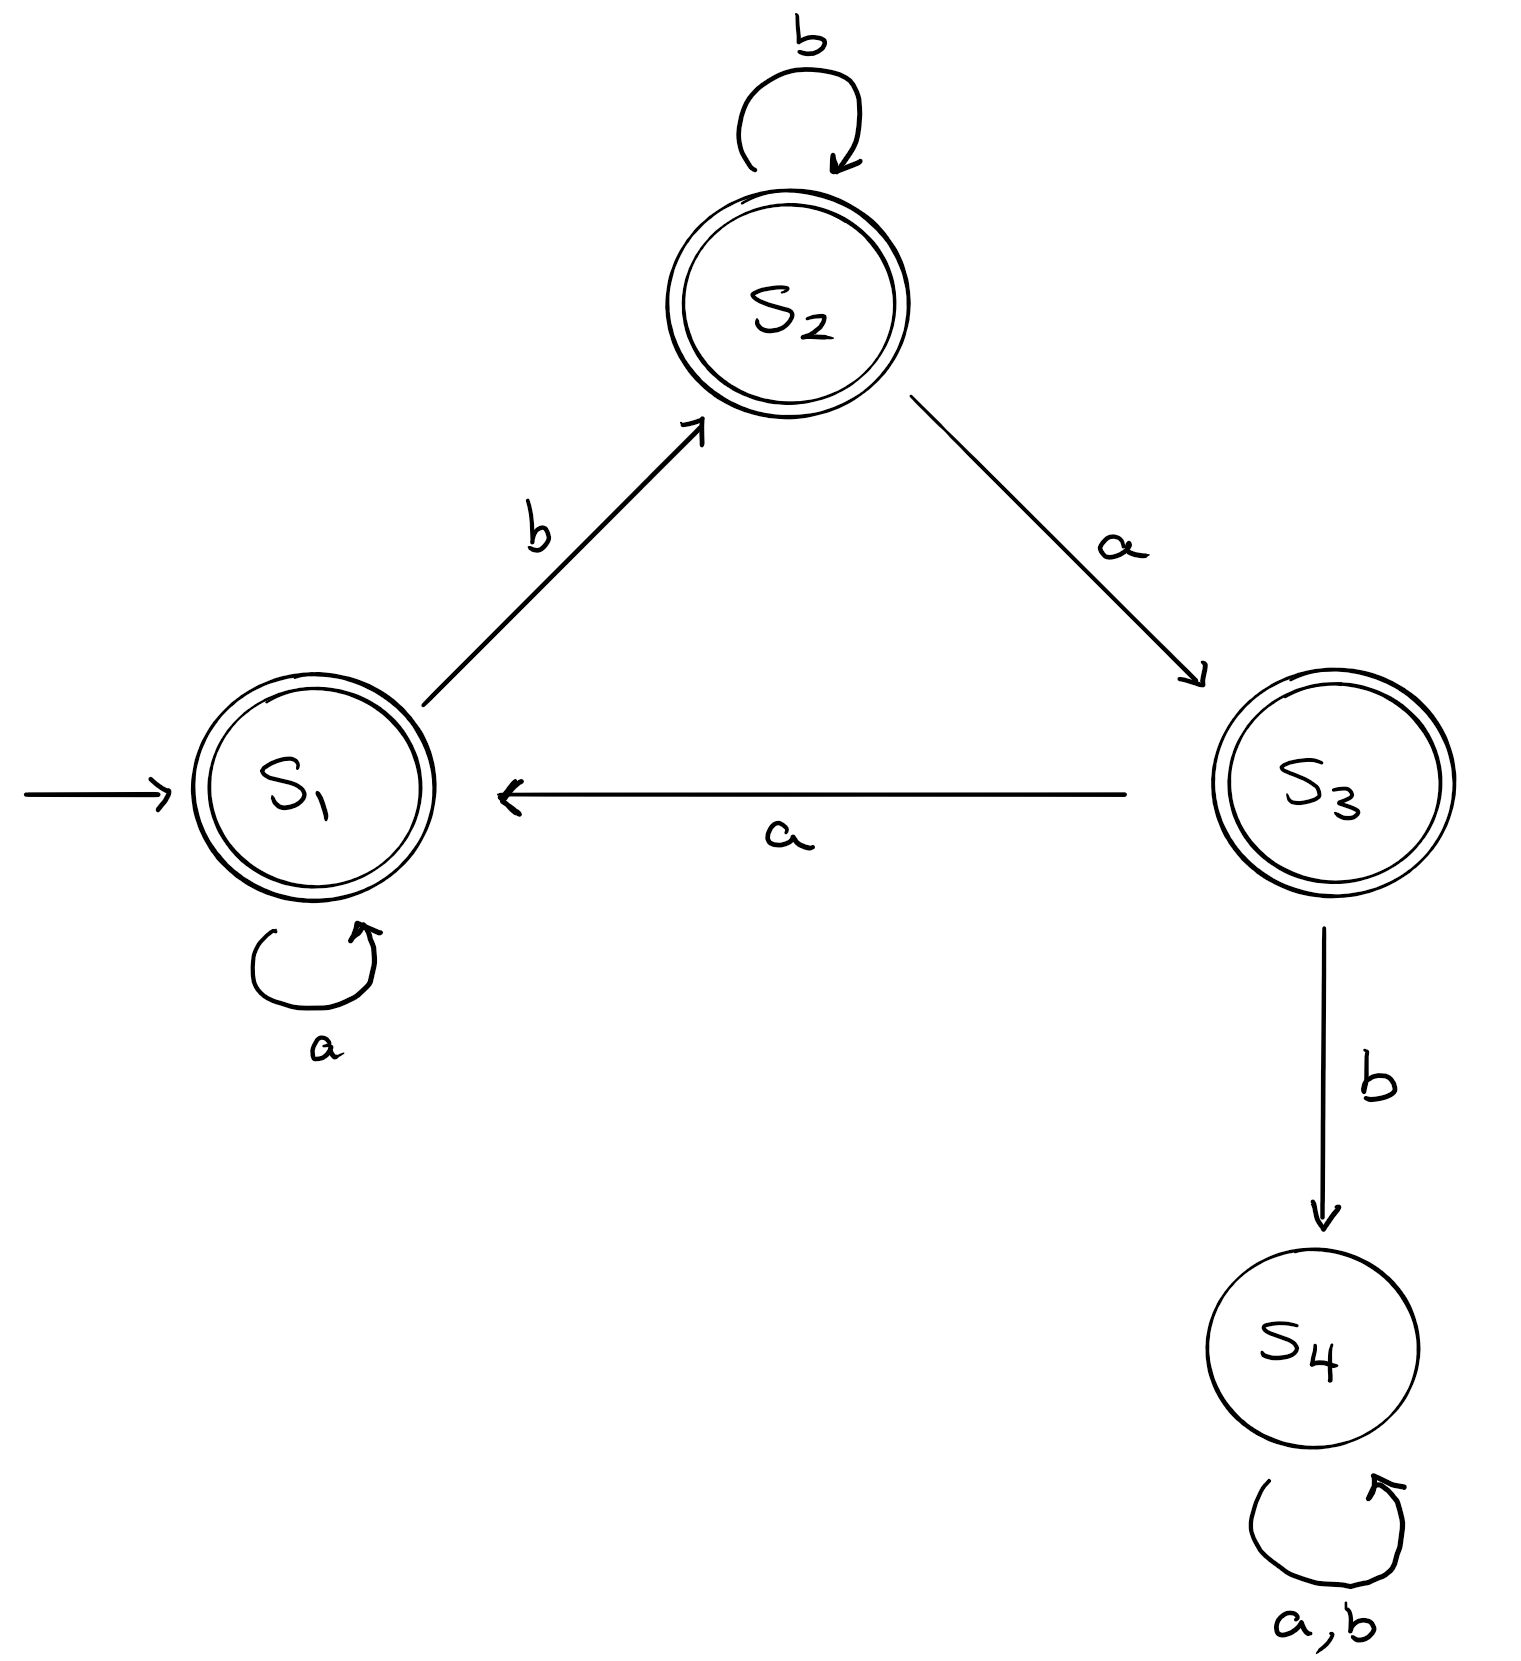
\includegraphics[scale = 0.2]{Word Acceptor.png}
			
			\label{fig5:sub1}
		\end{subfigure}%
		\begin{subfigure}{.3\textwidth}
			\begin{tabular}{c c}
				State	&	Current Word \\
				$S_1$	&	bbab \\
				$S_2$	&	\textcolor{green}{b}bab \\
				$S_2$	&	\textcolor{green}{bb}ab \\
				$S_3$	&	\textcolor{green}{bba}b \\
				$S_4$	&	\textcolor{green}{b}\textcolor{red}{bab} \\
				$S_2$	&	\textcolor{green}{b}aba \\
				$S_3$	&	\textcolor{green}{ba}ba \\
				$S_4$	&	\textcolor{red}{bab}a \\
				$S_1$	&	abaa \\
				$S_1$	&	\textcolor{green}{a}baa \\
				$S_2$	&	\textcolor{green}{ab}aa \\
				$S_3$	&	\textcolor{green}{aba}a \\
				$S_1$ & 	\textcolor{green}{abaa} \\
			\end{tabular}
		\end{subfigure}%
		\caption{The automaton $W$ that accepts any word which does not contain $bab$, and an example of reducing the word $bbab$ to the irreducible word $abaa$.}
	\end{figure*}
\end{example}

However, we may not be able to reduce all words with this process, as the left hand side of a rule may not appear directly in the word, but it may still be reducible.

\subsection{Knuth Bendix Algorithm}

FROM http://haskellformaths.blogspot.com/2010/05/string-rewriting-and-knuth-bendix.html

The \textbf{Knuth Bendix Algorithm} allows us to create new rules from out base set of rules, so that we can reduce every word in $A^*$ to a canonical element equal to it in $G$.

\begin{example}
	Consider the group $D_8 = \langle a, b | a^4, b^2, a^3 b = ba \rangle$ representing the symmetry group of the square. This gives us 3 rules for rewriting words:

	\begin{equation*}
		aaaa \to \varepsilon \hspace{3em}
		bb \to \varepsilon \hspace{3em}
		aaab \to ba
	\end{equation*}	

	From just these rules, we can reduce $abba$ to $aa$. However, we cannot reduce $bab$ or $aaa$, even though we know that they represent the same transformation of the square using the Cayley diagram for $D_8$. We could create a new rule connecting them immediately, however we need a way to tell that these two words do represent the same element just from the presentation.

	Consider the word $aaabb$. This can be reduced in two ways:

	\begin{gather*}
		aaabb \to bab \\
		aaabb \to aaa
	\end{gather*}

	Hence we know they must represent the same element, and can now formally add the rule $bab \to aaa$. 
\end{example}

We can do this more generally. Suppose there is a \textbf{critical pair}, which is a pair of two rules $L_1 \to R_1$ and $L_2 \to R_2$ such that there exists $A, B$ and $C$ such that:

$$ L_1 = AB \hspace{3em} L_2 = BC $$

Then we have the two reductions:

$$ ABC = L_1 C \to R_1 C $$
$$ ABC = AL_2 \to A R_2 $$

Hence we can add the rule $R_1 C \to A R_2 $. We repeat this process until there are no more critical pairs, at which point the set of rules is called \textbf{confluent}. Now we can construct the word acceptor $W$ which will reduce every word to a canonical element as in Example 5.3, allowing us to solve the word problem.

This differs from the Todd Coxeter Algorithm as it does not require us to enumerate all of the elements in the group, only enough rules to be able to reduce every element. Therefore, this algorithm is able to terminate for infinite groups, and so works on a larger category of groups.


% -------------------------------------------------------------

\section{Conclusion}

The Word Problem for groups is a difficult problem to solve in general, the ability to add graphs and automata to groups allows us to solve computational problems efficiently, and is not obvious from the definition of the group. Whilst the undecidability of the Uniform Word Problem is disappointing, a surprising number of useful and important groups admit polynomial time solutions to their Word Problem. Additionally it was one of the first algebraic, rather than logical or algorithmic, problems that was shown to be unsolvable, and so led to many other discoveries about unsolvable problems in algebra.

% -------------------------------------------------------------

\end{multicols}

\medskip

\begin{thebibliography}{9}
	\bibitem{Dehn}
	M. Dehn. 
	Über unendliche diskontinuierliche Gruppen.
	Mathematische Annalen, 71 (1): 116–144 (1911)

	\bibitem{Novikov}
	P. S. Novikov. 
	Uber die algorithmische Unentscheidbarkeit des Wortproblems in der Gruppentheorie. 
	Tr. Mat. Inst. Steklova 44, 140 S. (1955)

	\bibitem{RegularWords}
	I. A. Stewart, R. M. Thomas
	Formal Languages and the Word Problem for Groups.
	\\\texttt{https://community.dur.ac.uk/i.a.stewart/Papers/formallanguages.pdf}

	\bibitem{ToddCoxeter}
	K. Miller
	The Todd-Coxeter Algorithm
	\url{https://math.berkeley.edu/~kmill/notes/todd_coxeter.html}



\end{thebibliography}

\end{document}